\documentclass[a4paper,10pt]{article}
\usepackage{graphicx,wrapfig,hyperref}
\usepackage[hmargin=3.5cm,vmargin=3.0cm]{geometry}
\usepackage{glossary}
\makeglossary

% GLOSSARY
% eerst pdf maken
% dan dit uitvoeren in je terminal: makeindex requirements.glo -s requirements.ist -t requirements.glg -o requirements.gls
% dan nog een keer pdf maken

% Automatisch labelen van sections
\newcommand{\rsection}[1]{
\section{#1}\label{sec:#1}
}
\newcommand{\rsubsection}[1]{
\subsection{#1}\label{sec:sub:#1}
}
\newcommand{\rsubsubsection}[1]{
\subsubsection{#1}\label{sec:sub:sub:#1}
}

% Deze counter is voor requirements, ipv \item gebruik je \reqitem{req naam}.
% Om te referencen naar deze requirement schrijf je \reqref{req naam}.
\newcounter{rreqno}
\setcounter{rreqno}{0}
\newcommand{\rreq}[1]{\refstepcounter{rreqno}\label{#1}}
\newcommand{\reqitem}[1]{\rreq{#1}\item[(req \therreqno)]}
\newcommand{\reqref}[1]{requirement \ref{#1}}

% Use Cases
\newcommand\addrow[2]{#1 &#2\\ }

\newcommand\addheading[2]{#1 &#2\\ \hline}
\newcommand\tabularhead{\begin{tabular}{| lp{12cm} |}
\hline
}

\newcommand\addmulrow[2]{ \begin{minipage}[t][][t]{2.5cm}#1\end{minipage}% 
   &\begin{minipage}[t][][t]{8cm}
    \begin{enumerate} #2   \end{enumerate}
    \end{minipage}\\ }

\newenvironment{usecase}{\tabularhead}{\hline\end{tabular}}
% End use cases

\begin{document}

\title{TI2800 Contextproject - My Cultural Heritage\\ Requirements Analysis and Design}
\author{Sjoerd van Bekhoven\\ Tim Eversdijk \\ Herman Blanken \\ Rutger Plak \and 4014774 \\ 4005562 \\ 4078624 \\ 1358375}

\maketitle
\setcounter{page}{0}
\thispagestyle{empty}
\vspace{10cm}
\begin{figure}[ht!]
	\centering
	
\includegraphics[width=\textwidth]{cultuurapp-logo.png}
\end{figure}
\clearpage
\clearpage
\tableofcontents

\clearpage
\rsection{Introductie}
Het systeem \glossary{name={Systeem},description={de backend en\/of frontend}} zal toeristen \glossary{name={Toerist},description={een niet-ingelogde gebruiker van het systeem}} op een aantrekkelijke manier van zo nuttig mogelijke informatie voorzien van verschillende monumenten. Het systeem verreikt de kennis van toeristen en toont hen informatie die zij zonder het systeem niet te weten zouden zijn gekomen. Deze doelen zullen op verschillende manieren worden bereikt. De methoden die gebruikt zullen worden om deze doelen te verwezelijken staan beschreven \ref{sec:Functional requirements}.

\rsection{Overzicht}
	\rsubsection{Front-end}
\glossary{name={Front-end},description={het deel van het systeem dat zichtbaar is voor de toerist}}
	De front-end van de applicatie focust zich op twee punten:
	\begin{enumerate}
		\item Het aantrekkelijk weergeven van de informatie die we vergaard hebben van de monumenten.
		\item Het systeem zo intu\"itief mogelijk laten werken en weergeven.
	\end{enumerate}
				
	\rsubsection{Back-end}
\glossary{name={Back-end},description={het deel van het systeem dat niet zichtbaar is voor de toerist}}
	De back-end focust zich op het vergaren van nieuwe informatie voor ons systeem. Dit gebeurt op meerdere manieren:
	\begin{itemize}
		\item Niet alle monumenten hebben standaard een categorie aan zich gelinkt. De back-end zal door middel van beeld- en tekstanalyse bepalen in welke categorie het monument ingedeeld moet worden.
		\item Foto's van de monumenten zullen van Flickr en Wikimedia Commons gehaald worden.
\glossary{name={Wikimedia Commons},description={website waar miljoenen multimedia bestanden verzameld zijn, welke door iedereen vrij te gebruiken zijn}}
\glossary{name={Flickr},description={een website waarop mensen foto's kunnen uploaden en delen}}
		\item Data en foto's worden via de API \glossary{name={API},description={een schil die functies en data van het desbetreffende systeem beschikbaar stelt voor de buitenwereld via gedocumenteerde functies
}} van rijksmonumenten.nl opgehaald.
		\item Er wordt user-interactie-informatie bijgehouden.
		\item User-interactie-informatie wordt verwerkt tot bruikbare informatie, zoals bijvoorbeeld voorkeuren van users of applicatie brede aanbevelingen en sorteringen.
	\end{itemize}

\rsection{Functional requirements}
\rsubsection{Weergaves}
	\rsubsubsection{Kaart}
	\begin{enumerate}
		\reqitem{overview-maps} Het systeem moet de gefilterde monumenten (beschreven in \ref{sec:sub:Filtering}) als spelden weergeven op een Google Maps\footnote{\label{googlemaps} http://code.google.com/apis/maps/index.html} kaart.	
		\reqitem{overview-gps} Het systeem moet de locatie van de de toerist op de Google Maps$^{\ref{googlemaps}}$ kaart aangeven, mits deze beschikbaar is. 
	\end{enumerate}
	
	\rsubsubsection{Overzichtsweergave} \label{sec:views-detail}
	\begin{enumerate}
		\reqitem{overview-list} De overzichtsweergave toont een lijst met op iedere rij een monument.
		\reqitem{overview-info} Bij ieder monument staat een thumbnail, de titel, een korte beschrijving en categorie\"en.
		\reqitem{overview-click} Wanneer de toerist op een rij klikt komt hij op de detailpagina.
\reqitem{overview-order-filter} De getoonde set monumenten wordt bepaald door de door de toerist gekozen filtering en sortering als beschreven in \ref{filtering} \& \ref{sortering}.
	\end{enumerate}
	
	\rsubsubsection{Detailpagina} \label{sec:views-detail}
	\begin{enumerate}
		\reqitem{detail-info} De detailpagina toont de naam, omschrijving, afbeelding, locatie, provincie, gemeente, stad, postcode en de categorie van het monument.
		\reqitem{detail-flickr} De detailpagina toont Flickrfoto's uit de buurt van het monument. Zie ook \ref{sec:sub:Zoeken van relevante Flickr-foto's}.
		\reqitem{detail-4sq} \label{views-checkins} De detailpagina toont het recente aantal checkins op Foursquare. Zie ook \ref{sec:sub:Foursquare}.
\glossary{name={Foursquare},description={een website waarop mensen hun locatie kunnen delen}}
		\reqitem{detail-weather} De detailpagina toont de weersverwachting rond het monument. Zie ook \ref{sec:sub:Weersinformatie}.
		\reqitem{detail-places} De detailpagina toont faciliteiten in de buurt van het monument in een kaartje. Zie ook \ref{sec:sub:Faciliteiten rond monument-locatie}.	
\reqitem{detail-places-select} De toerist heeft de mogelijkheid om te selecteren welke faciliteiten rondom de monument-locatie worden getoond.
\reqitem{detail-analyse} De detailpagina toont visueel gelijkende monumenten. Zie ook \ref{sec:sub:Monumenten vergelijken aan de hand van foto's}.
		\reqitem{detail-favorize} De detailpagina bevat een knop waarmee een CultuurApp-gebruiker het monument aan zijn favorietenlijst kan toevoegen. Zie ook \ref{sec:sub:Favorieten toevoegen}.	
\end{enumerate}

\rsubsection{Filtering}
\label{filtering}
\begin{enumerate}
	\reqitem{filter-distance} Toeristen kunnen monumenten filteren op een bepaalde afstand van een zoeklocatie\footnote{\label{zoeklocatie}De zoeklocatie is een tekstvak op de webpagina waar een locatie in de vorm van een adres of door google maps herkende plaatsaanduiding kan worden ingegeven. Deze kan eventueel automatisch worden ingevuld met de locatie die de browser aanbiedt.}.
	\reqitem{filter-keywords} Toeristen kunnen monumenten filteren op trefwoorden.	
	\reqitem{filter-year} Toeristen kunnen monumenten filteren op bouwjaar.
	\reqitem{filter-category} Toeristen kunnen monumenten filteren op de categorie\"en uit de dataset.
\glossary{name={Dataset},description={de set van $\sim$25.000 monumenten die is vrijgegeven voor dit project}}
	\reqitem{filter-limit} Toeristen kunnen de lengte van de lijst met monumenten limiteren. De monumenten met de hoogste sortering blijven dan staan.
\end{enumerate}
		
\rsubsection{Sortering}
\label{sortering}
\begin{enumerate}
\reqitem{sort-popularity} Toeristen kunnen monumenten sorteren op populariteit.
\reqitem{sort-distance} Toeristen kunnen monumenten sorteren op afstand vanaf de gegeven zoeklocatie$^{\ref{zoeklocatie}}$.
\reqitem{sort-year} Toeristen kunnen monumenten sorteren op bouwjaar.
\end{enumerate}

\rsubsection{Foursquare}
\begin{enumerate}
	\reqitem{4sq-check} Het systeem kan controleren of er voor een monument een FourSquare 'venue' (de naam van een locatie op FourSquare) bestaat.
	\reqitem{4sq-make} Het systeem kan een FourSquare venue aanmaken indien dit voor een monument nog niet bestaat.
	\reqitem{4sq-checkins} De website toont het aantal check-ins bij de venue (zie ook \reqref{views-checkins}).
	\reqitem{detail-4sq} De website slaat bij het bezoeken van de detailpagina van een monument het meest recente aantal check-ins op FourSquare op.
	\reqitem{harvest-4sq} Een beheerder kan voor een hele set toegevoegde monumenten FourSquare locaties aan laten maken en check-ins laten controleren. Dit kan ook ingepland worden.
\end{enumerate}
                
\rsubsection{Weersinformatie}
\begin{enumerate}
	\reqitem{harvest-weather} Er is een systeemcomponent welke live door middel van het meegeven van de longitude en latitude van een locatie de weersverwachting voor deze locatie kan ophalen van Wunderground\footnote{http://dutch.wunderground.com/weather/api/}. 
\end{enumerate}
                
\rsubsection{Faciliteiten rond monument-locatie}
\begin{enumerate}
	\reqitem{harvest-places} Er is een systeemcomponent welke door middel van het meegeven van een longitude en latitude van een locatie en een faciliteit categorie faciliteiten in de buurt van deze locatie bij Google Places kan ophalen.
\end{enumerate}
                
\rsubsection{Monumenten vergelijken aan de hand van foto's}
\begin{enumerate}
	\reqitem{analyse-online-use} Het systeem kan zoeken in de resultaten van de Visuele Analyse (zie \ref{sec:sub:Visuele analyse} om bij \'e\'en afbeelding van een monument andere afbeeldingen te vinden die visueel gelijkend zijn.
\end{enumerate}

\rsubsection{Zoeken van relevante Flickr-foto's}
\begin{enumerate}
	\reqitem{harvest-flickr} Er is een systeemcomponent dat live foto's kan ophalen van Flickr\footnote{http://www.flickr.com/services/api/} aan de hand van de geografische locatie en textuele vergelijking van tags. Zie ook \ref{sec:sub:Textuele analyse}
\end{enumerate}
			
\rsubsection{Inloggen en registreren}
Toeristen kunnen inloggen met behulp van inlogsystemen van derden. OpenID en Facebook zullen in ieder geval worden ondersteund. Dit verlaagt de drempel voor het maken van een account omdat een toerist geen extra gegevens hoeft te onthouden.
\begin{enumerate}
	\reqitem{login-fb} Een toerist kan op het systeem inloggen via hun Facebook account.
	\reqitem{login-openid} Een toerist kan op het systeem inloggen via hun OpenID account.
	\reqitem{login-capp1} Een toerist kan een eigen CultuurApp-account aanmaken op het systeem door hun email adres en een wachtwoord in te vullen.
	\reqitem{login-capp2} Een toerist kan op het systeem inloggen met hun CultuurApp-account. 
\end{enumerate}

\rsubsection{Foto's toevoegen}
De CultuurApp-gebruiker moet foto's kunnen toevoegen van een monument.
\begin{enumerate}
	\reqitem{upload} Een CultuurApp-gebruiker kan een foto uploaden naar het systeem en daarbij aangeven om welk monument het gaat
	\reqitem{upload-desc} Een CultuurApp-gebruiker kan een beschrijving meegeven aan de geuploadde foto.
	\reqitem{upload-keywords} Een CultuurApp-gebruiker kan trefwoorden meegeven aan de ge\"uploadde foto.
	\reqitem{upload-delete} Een beheerder moet een ge\"uploadde foto kunnen verwijderen uit het systeem.
\end{enumerate}

\rsubsection{Favorieten toevoegen}
\begin{enumerate}
	\reqitem{favorize-detail-favorize} Een CultuurApp-gebruiker kan monumenten toevoegen aan zijn favorietenlijst. Zie ook \reqref{detail-favorize}.
	\reqitem{defavorize} Een CultuurApp-gebruiker kan monumenten verwijderen aan zijn favorietenlijst.
	\reqitem{favorize-public} Een CultuurApp-gebruiker kan zijn favorietenlijst openbaar maken.
	\reqitem{favorize-private} Een CultuurApp-gebruiker kan zijn favorietenlijst prive maken.
\end{enumerate}

\rsubsection{Gebruikers interactie}
\begin{enumerate}
	\reqitem{harvest-interaction-information-1} Het systeem houdt voor elke toerist bij welke foto's en detail pagina's van een monument worden bekeken.
	\reqitem{harvest-interaction-information-2} Het systeem houdt voor elke toerist bij welke filter criteria worden gebruikt.
	\reqitem{link-interaction-information} Wanneer een toerist inlogt en dus een CultuurApp-gebruiker is geworden wordt de eerder verzamelde informatie ook gekoppeld aan de CultuurApp-gebruiker.
\end{enumerate}

\rsubsection{Visuele analyse}
\begin{enumerate}
	\reqitem{visuele-analyse-offline} De foto's van alle monumenten uit de dataset worden offline visueel geanalyseerd me thet programma ImageJ\footnote{http://rsbweb.nih.gov/ij/} met de plugin ImagePlot\footnote{http://lab.softwarestudies.com/p/imageplot.html}.
	\reqitem{visuele-analyse-upload} De resultaten van de offline visuele analyse worden ge\"exporteerd en ge\"upload naar de database op de webserver.
\end{enumerate}

\rsubsection{Textuele analyse}
\begin{enumerate}
 	\reqitem{text-analyse} Er is een systeemcomponent dat textuele analyse uitvoert.
 	\reqitem{text-analyse-online} Dit systeemcomponent kan teksten analyseren met Naive Bayesiaanse filters. Indien er een dienst wordt gevonden die dit kan doen (uClassify.com is een kandidaat) dan wordt deze gebruikt, zo niet dan wordt dit ge\"implementeerd.
 	\reqitem{text-analyse-thesau} Dit systeemcomponent kan lexicografisch gelijkende woorden vinden met een Thesaurus. Zie \ref{sec:sub:Thesaurus}.
\end{enumerate}
    	                
\rsubsection{Thesaurus}
\begin{enumerate}
	\reqitem{thesau} Het systeem bevat een component welke een Thesaurus bevat, bijvoorbeeld Cornetto.
	\reqitem{thesau-getter} Wanneer een component in het systeem de Thesaurus aanroept en een (lijst van) woord(en) geeft, zal een lijst van relevante woorden worden teruggegeven.
\end{enumerate}

\rsubsection{Completeren dataset}
\begin{enumerate}
	\reqitem{completing-dataset} Het systeem kan de categorie-specifieke informatie filteren uit de afbeeldingen en beschrijvingen van moumenten met behulp van visuele en textuele analyse. Zie ook \ref{sec:sub:Visuele analyse} en \ref{sec:sub:Textuele analyse}.
	\reqitem{completing-dataset-coupling} Het systeem kan met behulp van de verworven categorie-specifieke informatie de ongecategoriseerde monumenten indelen in een visueel en textueel gelijkende categorie.
\end{enumerate}


		
\clearpage

\rsection{Quality requirements}	
		 	 	 		
\begin{enumerate}			

\item{Toegankelijkheid}
	\begin{enumerate}
		\reqitem{toegankelijkheid-client} De client heeft slechts een webkit of Gecko internetbrowser met een javascript engine. Dit betekent dat het op iedere computer / handheld met een gerenomeerde webbrowser (Google Chrome, Mozilla Firefox, Safari) werkt. Op een handheld device, zoals een iPhone of Android toestel, zal het systeem ook werken. 
		\reqitem{toegankelijkheid-locatie} Een toerist kan het systeem thuis gebruiken, maar ook op locatie (mits verbonden met internet).
\end{enumerate}

\item{Prestaties / Efficientie}
\begin{enumerate}	
		\reqitem{perf-php} 
	\reqitem{perf-js} De client berekent zelf de weergaves en de server wordt hier niet mee belast. Op deze manier wordt voorkomen dat kostbare resources worden verspilt.
\end{enumerate}

\item{Onderhoudbaarheid}
	\begin{enumerate}
		\reqitem{maint-pieces}Alle verbindingen met externe of interne data wordt aan de hand van kleine stukken code gemaakt. Deze kleine stukken code zijn eenvoudig te onderhouden.
		\reqitem{maint-repo}De updates kunnen eenvoudig op de webserver worden geinstalleerd door een nieuwe checkout van de code-repository te doen.
		\reqitem{maint-lokaal}Het lokaal ontwikkelen maakt het mogelijk nieuwe software uitvoerig te testen voor het online te zetten.
	\end{enumerate}

\item{Betrouwbaarheid en beschikbaarheid}
\begin{enumerate}
	\reqitem{avail-git} Door de manier van ontwikkelen is de server bij het updaten van de server slechts luttele seconden offline.
	\reqitem{relia-test} De betrouwbaarheid van de updates wordt gegarandeerd door de update eerst uitvoerig te testen op lokale systemen die hetzelfde zijn geconfigureerd als de webserver.
	\reqitem{avail-extern} Door het gebruik van verschillende externe databron valt bij het niet beschikbaar zijn van zo'n databron slechts (een deel van) een module uit.
	\reqitem{avail-maps} De kaarten Google Maps$^{\ref{googlemaps}}$ zijn een kritiek component, indien Google Maps niet beschikbaar is, is het systeem onbruikbaar. Google Maps heeft echter een up-time van minimaal 99,9\%\footnote{http://www.google.com/enterprise/earthmaps/maps-sla.html}. Dat komt neer op maximaal 90 seconden per dag, in de praktijk merkt een toerist hier niets van.
\end{enumerate}

\item{Security} 
\begin{enumerate}
\reqitem{sec-SQL} Het framework Kohana voorkomt sql-injections wanneer queries worden geseraliseerd via dit framework.
\reqitem{sec-} 
\end{enumerate}
\item{Precisie and Accuraatheid} 
	\begin{enumerate}
		\reqitem{prec-aanbevelingen} De aanbevelingen worden door het systeem op volgorde van relevantie getoond. Wanneer toeristen consequent niet de nummer 1 aanbeveling van een monument aanklikken, zal dit betekenen dat de aanbeveling niet correct is.
\end{enumerate} 
\end{enumerate}

\rsection{Design requirements}	

\begin{enumerate}		 	 	 		
\item{Constraints based on the type of users} 
	\begin{enumerate}
		\reqitem{upload-CA-user} CultuurApp-gebruikers kunnen foto's uploaden.
		\reqitem{upload-tourist} Toeristen kunnen geen foto's uploaden.
		\reqitem{favorites-CA-user} CultuurApp-gebruikers kunnen een favorietenlijstje bijhouden.
		\reqitem{favorites-tourist} Toeristen kunnen geen favorietenlijstje bijhouden.
		\reqitem{recom-CA-user} CultuurApp-gebruikers krijgen recommendation gebaseerd op hun eerder verzamelde data en dus ook van voorgaande bezoeken aan het systeem.
		\reqitem{recom-tourist} Toeristen krijgen of geen recommendation of recommendations gebaseerd op hun net verzamelde data.
	\end{enumerate}

\end{enumerate}
	
\rsection{Process requirements}	

\begin{enumerate}
		 	 	 		
\item{Ontwikkelingsmethode}
	\begin{enumerate}
		\reqitem{methodology} SCRUM wordt gebruikt bij het ontwikkelen van het systeem.
	\end{enumerate}
\item{Kosten en opleveringsdatum}
	\begin{enumerate}
		\reqitem{dev-enddate} Het systeem wordt 15 juni 2012 opgeleverd.
		\reqitem{dev-costs} Het systeem wordt gratis opgeleverd.
	\end{enumerate}
\item{Documentation}

\end{enumerate}

	\rsubsection{Constraints}
	\begin{itemize}
		\reqitem De back-end van de software zal draaien op een Debian Linux machine met een Apache webserver. Visuele gelijkenissen en verschillen worden onderzocht met de objectgeori\"enteerde programmeertaal Java. De data zal worden opgeslagen in een (My)SQL database. Voor het afhandelen van verzoeken van de client wordt de programmeertaal PHP gebruikt.
		\reqitem Aan de kant van de client wordt data opgehaald in HTML formaat. Hierin wordt de website opgebouwd met behulp van CSS. Om dynamisch dingen op de site te tonen of veranderen wordt JavaScript gebruikt.
\end{itemize}
		
	\clearpage
	\rsection{Analysis models}
	\rsubsection{Use case models,descriptions and scenarios}
		\rsubsubsection{Use case: selecteren}
		\begin{usecase}
		\addheading{Actor}{Toerist} g
			\addrow{Doel}{Het doel is de toerist op een eenvoudige wijze monumenten te laten zoeken aan de hand van verschillende criteria. De toerist moet aan de hand van zijn interesses de hoeveelheid monumenten verlagen zodat eenvoudig de interesses naar voren komen in de getoonde monumenten.}
			\addrow{Triggers}{Deze use case wordt getriggerd zodra de toerist een of meerdere selectiecriteria invult.}
			\addrow{Preconditie}{De set met getoonde monumenten is de set van alle monumenten.}
			\addrow{Postconditie}{De input van de toerist wordt omgezet naar een set monumenten die aan de selectie voldoen. In de kaartweergave zal dit betekenen dat de hoeveelheid spelden verminderd. In de overzichtsweergave zal dit betekenen dat de hoeveelheid informatierijen verminderd.}
			\addrow{Samenvatting}{"Als toerist wil ik aan de hand van verschillende selectiecriteria de monumenten in de resultaatpagina beperken:
				\begin{itemize}
					\item Wanneer ik kaartweergave gebruik, moeten spelden verdwijnen of verschijnen afhankelijk van of de monumenten die deze spelden verantwoorden aan deze selectiecriteria voldoen.
					\item Wanneer ik overzichtsweergave gebruik, moeten rijen informatie verdwijnen of verschijnen afhankelijk vam of de monumenten die deze rijen informatie verantwoorden aan deze selectiecriteria voldoen."
				\end{itemize}
			}
			\end{usecase}

			\rsubsubsection{Use case: informatie}
			\begin{usecase} 
			\addheading{Actor}{Toerist} 
			\addrow{Doel}{Het doel is de toerist op een overzichtelijke en natuurlijke manier van informatie over het geselecteerde monument te voorzien. De toerist moet nuttige informatie te zien krijgen. Ook moet hij informatie te zien krijgen die hem kunnen helpen bij het bezoeken van het monument.}
			\addrow{Triggers}{Deze use case beschrijft de situatie waarin de toerist een monument selecteert. In de overzichtsweergave gebeurt dit wanneer een informatierij die een monument vertegenwoordigt aangeklikt wordt. In de kaartweergave gebeurt dit bij het aanklikken van een speld die een monument vertegenwoordigt.}
			\addrow{Preconditie}{De toerist weet niets van het geselecteerde monument.}
			\addrow{Postconditie}{De toerist weet veel over het monument en heeft alle informatie die de toerist nodig heeft wanneer de toerist het monument zou willen bezoeken.}
			\addrow{Samenvatting}{"Als toerist wil ik wanneer ik op een speld op de kaart, of informatierij in de overzichtsweergave klik, verwezen worden naar de pagina met informatie over het monument die de speld of informatierij verantwoord. Op deze pagina wil ik de informatie beschreven in figuur \ref{interface3} op pagina \pageref{interface3} te zien krijgen. Ik wil een kaartje te zien krijgen waarin is ingezoomd op het monument. Op de kaart wil ik in een straal van x kilometer hotels kunnen zoeken, evenals restaurants, barretjes en andere monumenten. Ik wil dat het systeem mijn interesses bepaald en aan de hand van mijn interesses monumenten aanraadt waar ik in ge\"interesseerd ben."}
			\end{usecase}	

			\rsubsubsection{Use case: mobiliteit}
			\begin{usecase} 
			\addheading{Actor}{Toerist} 
			\addrow{Doel}{De toerist op locatie voorzien van informatie en het mogelijk maken foto's toe te voegen aan het systeem.}
			\addrow{Triggers}{De toerist gebruikt zijn mobiele apparaat om een monument te selecteren. Dit kan aan de hand van de selectieprocedure beschreven in use case 1, maar ook aan de hand van een lijst favoriete monumenten die aangemaakt kan worden zoals beschreven in use case 4.}
			\addrow{Preconditie}{De toerist is onderweg en wil informatie opzoeken. De toerist heeft op zijn mobiele apparaat een internetverbinding waarmee de toerist het systeem kan raadplegen.}
			\addrow{Postconditie}{De toerist heeft op locatie toegang tot informatie. Het systeem heeft extra foto's.}
			\addrow{Samenvatting}{"Als toerist wil ik wanneer ik op de plaats van bestemming ben aangekomen met behulp van mijn mobiele apparaat een foto kunnen uploaden / twitteren die door het systeem wordt toegevoegd aan de foto's die bij het monument horen. Ik wil hierbij steekwoorden kunnen meegeven die door het systeem worden herkend. Wanneer ik via dit mobiele systeem een monument, hotel, bar, of ander point of interest selecteer, wil ik dat het navigatieprogramma van mijn mobiele apparaat automatisch opent, zodat ik hier eenvoudig naar toe geleid wordt."	}
			\end{usecase}

			\rsubsubsection{Use case: favorieten}
			\begin{usecase} 
			\addheading{Actor}{Toerist} 
			\addrow{Doel}{De toerist zijn favoriete monumenten eenvoudig terug te laten vinden.}
			\addrow{Triggers}{De toerist voegt een monument toe aan zijn favorieten.}
			\addrow{Preconditie}{De toerist heeft monumenten gevonden.}
			\addrow{Postconditie}{De toerist kan inloggen om zijn lijst favoriete monumenten te raadplegen.}
			\addrow{Samenvatting}{"Als toerist wil ik wanneer ik een monument heb gevonden dat ik graag zou willen bezoeken of op een later tijdstip nogmaals wil bekijken, dat ik dit monument aan een lijst kan toevoegen. Deze lijst wil ik altijd kunnen raadplegen na inloggen met mijn gebruikersnaam en wachtwoord of OpenID. Wanneer ik onderweg ben, wil ik op mijn mobiele apparaat kunnen inloggen en alle beschikbare informatie over dit monument kunnen zien. Wel wil ik zelf kunnen bepalen of andere toeristen mijn lijst met monumenten kunnen bekijken."}
			\end{usecase}	
			
			\rsubsubsection{Use case: toevoegen foto's}
			\begin{usecase}
			\addheading{Actor}{Toerist}
\addrow{Doel}{De toerist extra foto's laten toevoegen aan de database.}
\addrow{Triggers}{De toerist upload een foto.}
			\addrow{Precondities}{De toerist is bij het monument en maakt een foto.}
			\addrow{Post condities}{De foto is toegevoegd aan de database van foto's die bij het monument horen.}
			\addrow{Samenvatting}{"Als toerist wil ik als ik bij een monument ben een foto kunnen maken en deze op kunnen slaan in de database. Dit wil ik doen door vanuit de mobiele applicatie een foto te maken en te uploaden. Ook kan een toerist zodra hij of zij thuis komt foto's van een monument uploaden."}
			\end{usecase}
		
\rsubsection{Business object model}
		Het "Business object model" is het object model van ons systeem. Dit model is uitgebeeld in figuur \ref{bom}.
		\begin{figure}[ht!]
			\centering
			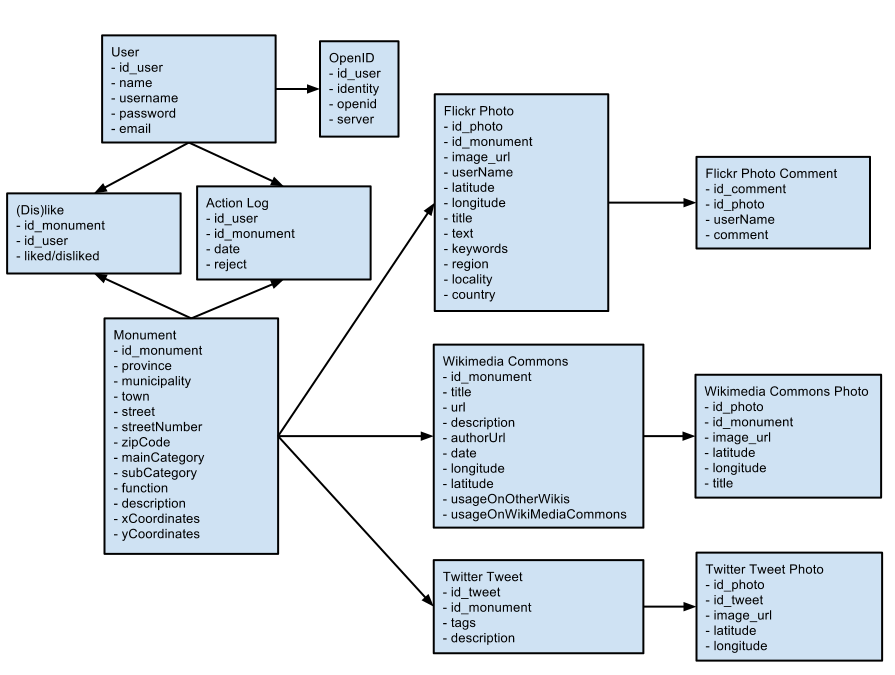
\includegraphics[width=\textwidth]{BusinessObjectModel.png}
			\caption{Business Object Model \label{bom}}
		\end{figure}
		\rsubsection{Dynamische modellen}
			\rsubsubsection{Overzichtspagina}
			In figuur \ref{sequence1} is beschreven hoe de overzichtspagina tot stand komt. Hierin is ook te zien hoe de informatie die op de kaart moet worden weergeven naar een externe server wordt gestuurd, waarna er een kaartje met spelden wordt teruggestuurd. Zie ook \ref{sec:sub:sub:Kaart} en \ref{sec:sub:sub:Overzichtsweergave}.
\begin{figure}[ht!]
				\centering
				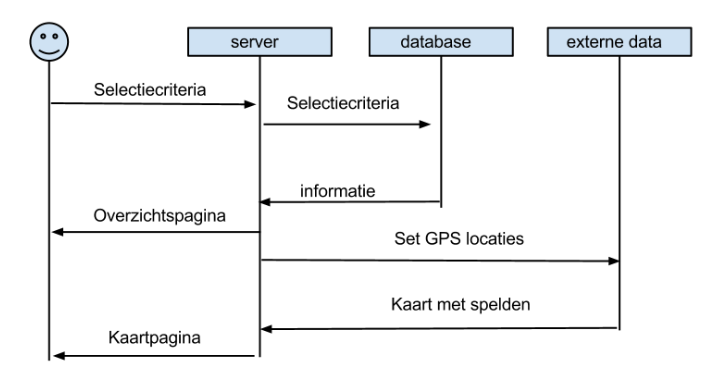
\includegraphics[width=\textwidth]{sequence1.png}
				\caption{Sequence Diagram 1 \label{sequence1}}
			\end{figure}
			\rsubsubsection{Sequence diagram 2}
			figuur \ref{sequence2}.
			\begin{figure}[ht!]
				\centering
				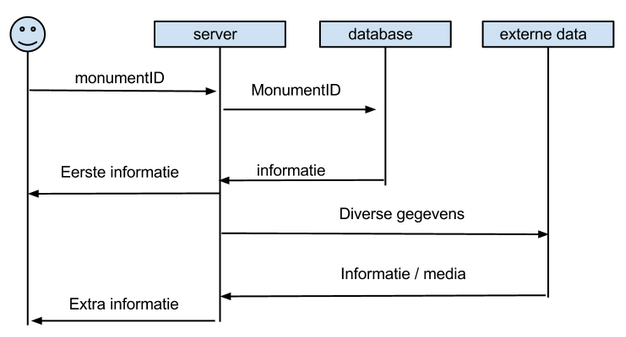
\includegraphics[width=\textwidth]{sequence2.png}
				\caption{Sequence Diagram 2 \label{sequence2}}
			\end{figure}		
		\clearpage			
		\rsection{User interface}
			\begin{figure}[ht!]
			\centering
			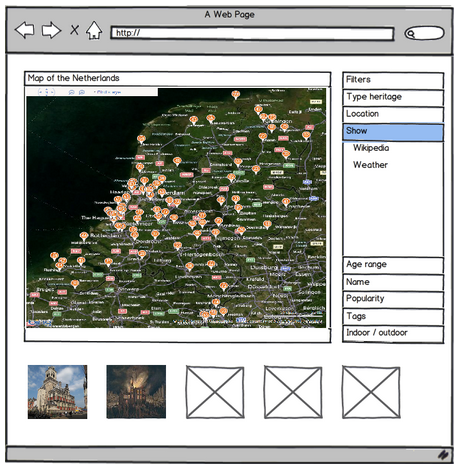
\includegraphics[height=10cm]{interface1.png}
			\caption{Kaart met monumenten \label{interface1}}
			\end{figure}
	
			\begin{figure}[ht!]
				\centering
				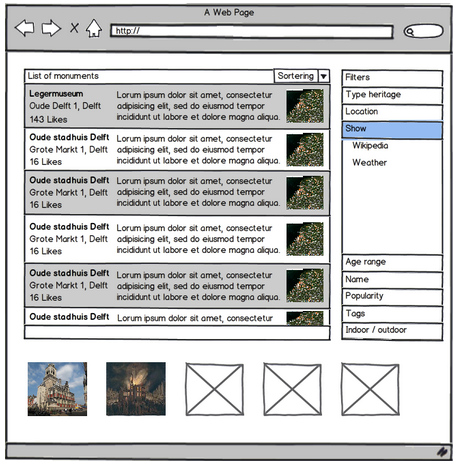
\includegraphics[height=10cm]{interface2.png}
				\caption{Overzichtspagina met monumenten \label{interface2}}
			\end{figure}
			\begin{figure}[ht!]
				\centering
				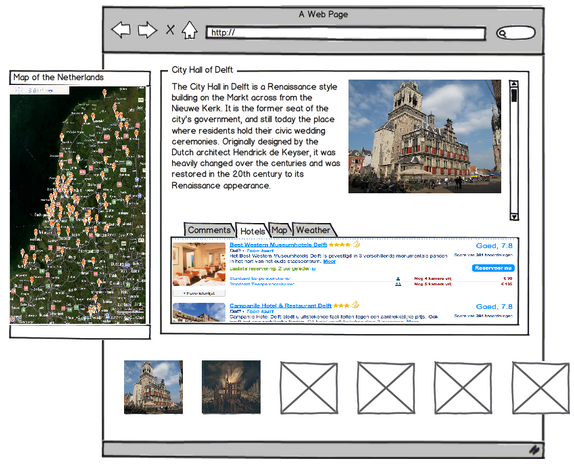
\includegraphics[height=10cm]{interface3.png}
				\caption{Detailpagina monument \label{interface3}}
			\end{figure}
	
	\clearpage

	\printglossary
\end{document}